\epigraph{The difference between ideas and reality is like the
difference between philosophy and engineering. The work to transform one into
the other is scientific research}{{\itshape V-Research}}

Several standards mandates a secure-by-design approach in which 
cybersecurity shall be considered at the very early stages of the 
design process. For example,
\begin{enumerate}[noitemsep]
	\item DO-326A -- ``Airworthiness Security Process Specification''
		requires a cybersecurity risk assessment of the design and is
		the ``are the only Acceptable Means of Compliance (AMC) by FAA
		\& EASA for aviation cyber-security airworthiness certification,
		as of 2019'' as pointed out by SAE in \autocite{SAE2019DO326A}.
	\item NIST 800-82 \autocite{Stouffer2011guide} -- ``guide to Industrial
		Control System (ICS) Security''
	\item J3061:2016-1 \autocite{SAE2016J3061} -- ``Cybersecurity Guidebook
		for Cyber-Physical Vehicle Systems'' defines ``set of
		high-level guiding principles for Cybersecurity as it relates
		to cyber-physical vehicle systems'' and states that
		``incorporate Cybersecurity into cyber-physical vehicle systems
		from concept phase through production, operation, service, and
		decommissioning''
\end{enumerate}
Companies who develop CPS (e.g. aerospace systems or elevator systems), must adhere
to strict regulations and quality assurances processes. Introducing tools and procedures 
in their processes requires a detailed and justified overview on how those
tools and procedures can be used. In Figure~\ref{fig:spdl}, we provide an overview
of a process that consider cybersecurity in the specification, design, and implementation
stages. The overall process start with the specification of the architectural (both physical
and functional) requirements from which the Weaknesses are automatically identified.
Based on the Assets, architectures, and the Weaknesses the cybersecurity risk is
calculated based on the $\abf$-theory. An iterative process between 
the user (e.g. the engineer) and the \secramod module of the \abftool allows the user to move to the design phase
when the risk level is considered acceptable. The design phase starts by automatically mapping
the Weaknesses into Vulnerabilities which are, in turn, fed into the \designverifmod
module along with the final specification. The Module returns a list of Vulnerabilities and
potential Mitigations. The user then procees in implementing the CPS and the SW/HW choices
can be tested by the \atgmod. 

\begin{figure}[t]
	\centering
	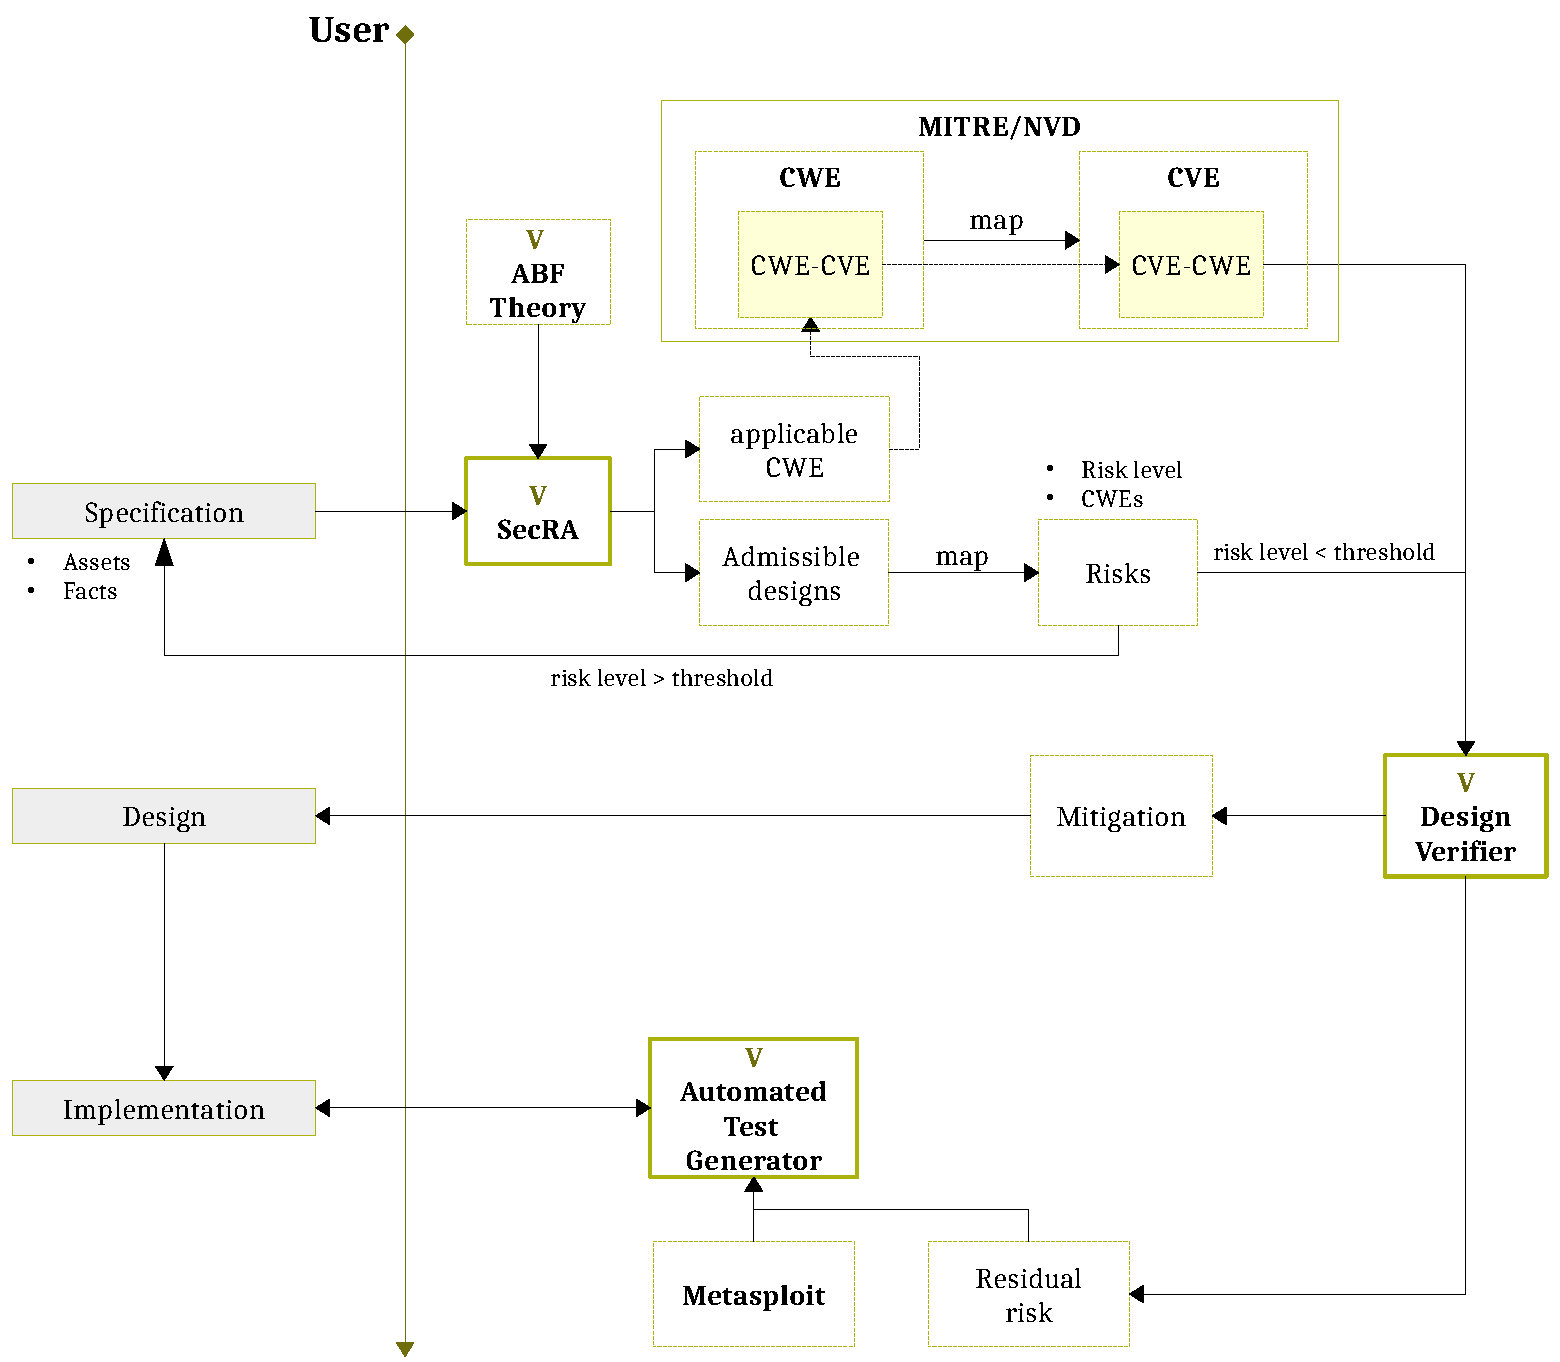
\includegraphics[width=\textwidth]{spdl.pdf}
	\caption{Secure-by-design System Development Life-cycle}
	\label{fig:spdl}
\end{figure}

In order to explain in details the SPDL, we use the following running example.
\begin{example}
	As depicted in Figure~\ref{fig:usecase}, the use case of the running example
	(a small part of a subprocess of the SwAT testbed \autocite{}), shows
	\begin{itemize}[noitemsep]
		\item a tank that is filled with raw water coming from the inlet pipe 
		\item a motorized valve (a valve with an actuator) that regulates that
			\begin{itemize}
				\item if opened, allows the raw water to flow into the tank
				\item if closed, stops the raw water to flow into the tank
			\end{itemize}
		\item a sensor that reads the meters of raw water in the tank
		\item a PLC controller, connected to the sensor and the actuator, that receives the readings from the sensor and regulates the quantity of water in the tank by communicating a change in the state of the actuator based on the following logi
			\begin{itemize}
				\item if the readings from the sensor reports a water level in the tank above (or equal) to 10m, the actuator shall close the valve
				\item if th readings are below 10m the actuator shall open the valve.
			\end{itemize}
	\end{itemize}

\begin{figure}[t]
	\centering
	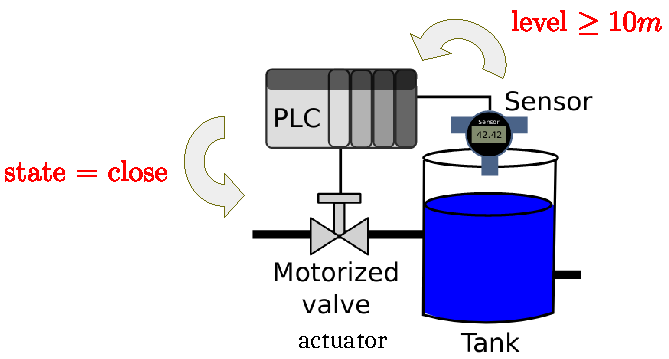
\includegraphics[width=.55\textwidth]{usecase.pdf}
	\caption{Use Case -- Running Example}
	\label{fig:usecase}
\end{figure}
\end{example}

\subsection{Specification -- Elicitation of Security Requirements}\label{sec:properties}
\begin{figure}[t]
	\centering
	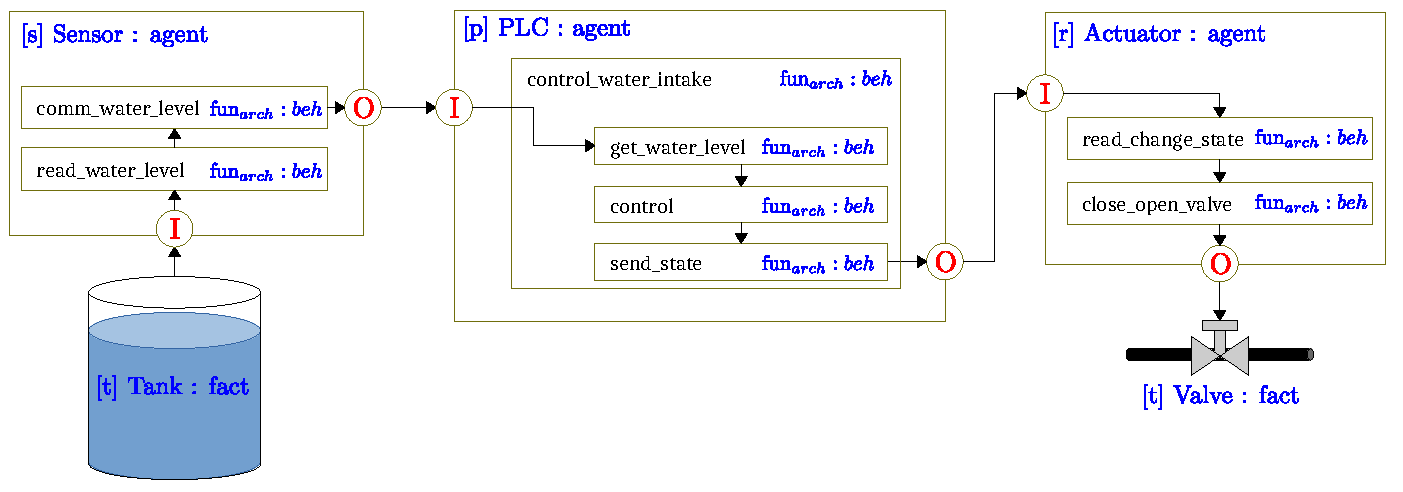
\includegraphics[width=\textwidth]{spec.pdf}
	\caption{Specification -- Running Example}
	\label{fig:spec}
\end{figure}
The first step of the SPDL is the definition of the requirements and then, for
the purpose of this paper of the (i) security requirements, (ii) architectural
(physical and functional) requirements.  Our focus in mainly on security
requirements but they are necessarily intertwined with the architectural
requirements, as we will show afterwards in this section.  A complete study on
how to properly define the architectural requirements is outside the scope of
this paper so we propose a method that is convenient for the purpose of our
assessment.

\Paragraph{System Requirements}
In our running example, there is a system (a CPS) composed by $5$ main
subsystem which we consider atomic (i.e. not themself composed by subsystems)
and then agents: the tank, the sensor, the controller, the actuator, and the
motorized valve (valve from now on).  The whole specification (which we now
describe) of the physical and functional architecture is depicted in
Figure~\ref{fig:spec}.  In the use case, the communication flow is as follows:
\begin{enumerate}
	\item the sensor reads the level of water in the tank ($\text{tank}\rightarrow \text{sensor}$) \footnote{this communication depends on the technology in use for the readings. We assume a unidirectional communication without loss of generality}
	\item the sensor communicates the readings to the controller ($\text{sensor}\rightarrow \text{controller}$)
	\item the controller calculates the valve state and communicates it to the actuator ($\text{controller}\rightarrow \text{actuator}$)
	\item the actuator translates (digital to analog) the states received and communicates\footnote{we do not distinguish, for the sake of simplicity between different types of channels and assume that communicating to the valve produces the expected change of physical state} it to the valve
\end{enumerate}
Each agent has an input or output port from which it communicates with other
agents.  It is also composed by the functional blocks that defines its
functional architecture and physical boundaries that defines its physical
architecture, as follows.
\begin{enumerate}[start=1, label={req\arabic*)}]
	\item the tank has no functional architecture, it is a purely physical component which has the only purpose of containing water
	\item the communication is unidirectional from the tank to the input port of the sensor
	\item the sensor has an input-port that receives only incoming communication from the tank
	\item the sensor has two functional blocks
		\begin{enumerate}[label={req4.\arabic*)}]
			\item read\_water\_level, accepts inputs only from the input-port and outputs a new reading every $t$ seconds
			\item comm\_water\_level, accepts inputs only from the read\_water\_level and communicates the readings to the output-port
		\end{enumerate}
	\item the sensor has an output-port that only outputs the messages generated by the comm\_water\_level to the input-port of the controller
	\item the controller has in input-port that only receives incoming communications from the sensor and sends the messages to the functional architecture
	\item the functional architecture of the controller is composed by three functional blocks
		\begin{enumerate}[label={req7.\arabic*)}]
			\item get\_water\_level, accepts inputs only from the input-port and outputs the water level to the main control function
			\item control, calculate the next state of the valve based on the inputs receive from the get\_water\_level
			\item send\_state, receives the output of the control function and communicates it to the output-port
		\end{enumerate}
	\item the controller has an output-port that only outputs the messages generated by the send\_state to the input-port of the actuator 
	\item the actuator has an input-port that receives only incoming communication from the controller 
	\item the functional architecture of the actuator is composed by two functional blocks
		\begin{enumerate}[label={req10.\arabic*)}]
			\item read\_change\_state, accepts inputs only from the input-port and outputs the next state of the valve to the close\_open\_valve function
			\item close\_open\_valve, converts the digital next state received from the read\_change\_state an analog signal and communicates it the output-port
		\end{enumerate}
	\item the valve accepts analog messages from the output port of the actuator and changes its state based on those messages
\end{enumerate}

\begin{figure}[t]
	\centering
	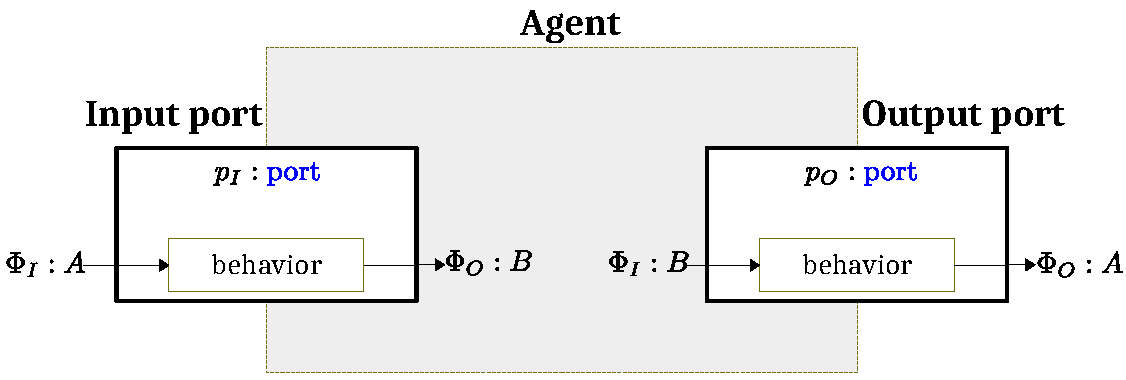
\includegraphics[width=.9\textwidth]{IOports.pdf}
	\caption{Input and Output Port of an agent}
	\label{fig:ioports}
\end{figure}

\begin{figure}[t]
	\centering
	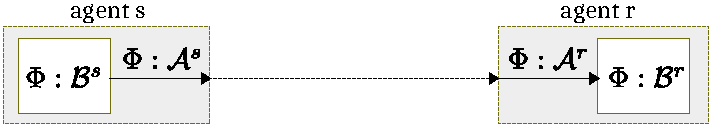
\includegraphics[width=.9\textwidth]{channel.pdf}
	\caption{Communication over a Mono-directional Channel}
	\label{fig:channel}
\end{figure}

While \emph{agents} and \emph{communication} between agents are described and
defined in Section~\ref{sec:theory}, the concepts of \emph{port} (depicted in
Figure~\ref{fig:ioports}), \emph{channel} (depicted in
Figure~\ref{fig:channel}), \emph{functional and physical architecture}, and
\emph{functional block} have not yet been defined with respect to the
$\abf$-theory.  Informally, a channel\footnote{for now, we rely on the
intuitive notion of channel as ``something'' that transfers information as
Assertions between output and input port, i.e. mono-directional} identifies the
place where the communication takes place.  In this work, we only consider
mono-directional channels and communication but the extension to bi-directional
channel can be considered as the union of two unidirectional channels. A
mono-directional channel is defined by the assertions sent or received (over
the channel). 

\Paragraph{Input and Output Ports}
Since the $\abf$-theory is a theory of agents, we consider ports as agents that
allows the exchange of information between a channel and another
agent.  However, a port must be considered as a special type of agent to avoid
an \emph{infinite regress} in which a port needs a port to transfer information
between the outside of the port to the inside of itself.

\begin{definition}{\bf Input or Output Port --}\label{def:port} 
	Ports are agents with the following predefined behavior: an input-port changes
	the type of information from assertion from a sender $s$ to an agent $a$,
	$\rassert{s}{a}$ to belief of the agent $a$ ($\beliefRegion_a$) while an
	output-port from belief to assertion; forwarding information from the outside
	of an agent's boundary to the inside (input-port) or vice versa (output-port). 
\end{definition}
The \emph{quality of a port} is determined by the $\rcc$ relation between the 
assertions received or sent and the belief, i.e. $\Rcc{\assertionRegion_s}{\beliefRegion_a}$ for the input-port
or $\Rcc{\assertionRegion_r}{\beliefRegion_a}$.

\begin{definition}{\bf Secure Input Port --}\label{def:secport}
	A secure input port allows information as incoming assertions to flow
	from a sender $s$ to the behavior of the recipient $a$ (agent).  If $p_I$ is a secure input port,
	$\world\models\varphi$, and $\varphi\in\assertionRegion_s$ where $s$
	has the only input port $p_I$, $\world'\models\beliefRegion_a$ and $\varphi\in\beliefRegion_a$.
\end{definition}

\Paragraph{Port Weaknesses}
From this definition, it follows that there exist only the following \emph{six} types of weaknesses, generating six types of insecure port in RCC5 (the notation is reported for input-ports, i.e. on the lef-hand side of the arrow):
\begin{enumerate}[start=1, label={W\arabic*)}]
	\item \emph{drop port} ($s\dropport a$), where assertions reaches the port but do not pass the boundary of the agent (i.e. do not become belief of the agent)
	\item \emph{insertion port} ($s\insertport a$), where some new information is believed by $a$ as incoming from the port but $s$ didn't send it
	\item \emph{injection port} ($s\injectionport a$), where information coming from $s$ is substituted with new information which becomes believed by $a$
	\item \emph{selective port}, where some information passes the port and part is either:
	\begin{enumerate}[start=1, label={W4.\arabic*)}]
		\item dropped ($s\selectivedropport a$), 
		\item inserted ($s\selectiveinsertport a$), or
		\item injected ($s\selectiveinjectionport a$)
\end{enumerate}
\end{enumerate}

\begin{proof}
An input port is, in the $\abf$-theory, defined secure as long as the relation
	between the two regions of input assertions $\assertionRegion$ and
	output beliefs $\beliefRegion$ are equal, i.e.
	$\eq{\assertionRegion}{\beliefRegion}$. Therefore, any other relation
	should result in a weakness (related to an insecurity flaw) of that
	input port.  Using RCC5, there exist exactly other $4$ different type
	of relations, one of which is the discrete-from (DR) relation, i.e.
	$\dr{\assertionRegion}{\beliefRegion}$. When two regions are related by
	the DR relations, they have no subregion in common. Lets
	define a function weight $|X|$ such as, for any region $X$, it
	represents the smallest possible cardinality of a (mereo)topological base for
	$X$; where a base is a collection of regions in a (mereo)topology such that
	every open region can be written as union of elements of that base.  If
	a communication occurred and results in
	$\dr{\assertionRegion}{\beliefRegion}$, there exist only two mutually
	exclusive options: either $|\assertionRegion|=|\beliefRegion|$ or
	$|\assertionRegion|\neq|\beliefRegion|$. 
	\begin{itemize}
		\item If $|\assertionRegion|\neq|\beliefRegion|$ (at the end of
			a communication through the input-port), the two
			regions have a different number of subregions, and,
			then, there exist only two mutually exclusive options: 
			\begin{itemize}
				\item either $|\assertionRegion|>|\beliefRegion|$, where one
					ore more Assertions didn't become Beliefs, which we
					call \emph{drop port} ($s\dropport a$) since its behavior drops and
					prevents incoming communications,
				\item or $|\assertionRegion|<|\beliefRegion|$, where there are
					one ore more Beliefs which have not been sent as
					input-Assertions, which we call \emph{insertion
					port} ($s\insertport a$) since its behavior generates new Beliefs
					unrelated to the incoming communication. 
			\end{itemize}
		\item If $|\assertionRegion|=|\beliefRegion|$, supposing an increasing monotonic entropy on the information (Assertions) exchanged, 
				there exist only two mutually exclusive options: 
			\begin{itemize}
				\item either information has been generated as Belief and transferred as Assertions, increasing the cardinality of both
					$\assertionRegion$ and $\beliefRegion$, i.e.
					$|\assertionRegion_{t^0}|>|\assertionRegion_{t^1}|$ and
					$|\beliefRegion_{t^0}|>|\beliefRegion_{t^1}|$ (where
					$t^0$ and $t^1$ represent time at the beginning of
					communication and right after, respectively); which
					means that Assertions have reached the port and new
					Beliefs have been generated by the port, but no
					correlation between the elements of the two regions exist. 
					We call this \emph{injection port} ($s\injectionport a$) since it has modified
					the information carried by the Assertions into new
					corresponding Beliefs.
				\item or $|\assertionRegion_{t^0}|=|\assertionRegion_{t^1}|$
					and $|\beliefRegion_{t^0}|=|\beliefRegion_{t^1}|$ but
					this implies that no communication occurred, while we
					assumed that a communication was taking place (absurd).
			\end{itemize}
	\end{itemize}
	In other words, $\dr{\assertionRegion}{\beliefRegion}\equiv\neg\overlaps{\assertionRegion}{\beliefRegion}\equiv\neg(\varphi\subseteq\assertionRegion\wedge\varphi\subseteq\beliefRegion)\equiv\varphi\not\subseteq\assertionRegion\vee\varphi\not\subseteq\beliefRegion$
	Similarly, 
	\begin{itemize}
		\item given that $\po{\assertionRegion}{\beliefRegion}$ is equivalent to
			$\dr{\assertionRegion}{\beliefRegion}$ except for the
			overlapping part (see Appendix~\ref{app:selectiveinjectionport}) in which case is
			$\eq{\assertionRegion}{\beliefRegion}$ (see
			\autocite{Santaca2016abf}),
			we call it a \emph{selective injection port} ($s\selectiveinjectionport a$); otherwise
		\item $\pp{\assertionRegion}{\beliefRegion}\equiv\assertionRegion\Leftarrow\beliefRegion$ and
			$\ppi{\assertionRegion}{\beliefRegion}\equiv\assertionRegion\Rightarrow\beliefRegion$ are subcases of
			$\eq{\assertionRegion}{\beliefRegion}\equiv\assertionRegion\Leftrightarrow\beliefRegion$, and then
		\begin{itemize}
			\item if $\pp{\assertionRegion}{\beliefRegion}$, we have that
				some Beliefs are not correlated to incoming Assertions
				and we call it \emph{selective insertion port} ($s\selectiveinsertport a$),
			\item if $\ppi{\assertionRegion}{\beliefRegion}$ we have that
				some incoming Assertions are not correlated to Belief 
				and we call it \emph{selective drop port} ($s\selectivedropport a$)
		\end{itemize}
	\end{itemize}
\end{proof}

\Paragraph{Communication Channels}
We start by considering the difference between a (communication)
mono-directional channel (channel from now on) and an agent, as we did for the
ports, since the $\abf$-theory is a theory of agents.  In fact, if a channel
were considered an agent (channel-agent) then the question would be how an
agent would transfer its Assertions to the channel-agent. If the channel
between the agent and the channel-agent is again an agent, we would generate an
\emph{infinite regress}. Therefore, we do allow channel-agents but we assume a
finite depth (of detail) for a channel, where there exists a bottom-channel
which is not an agent. For now, we do not constrain a channel-agent in any way
so there is no difference between a channel agent and agent. Therefore, for the
sake of simplicity, we consider, in this text, channels to be bottom-channels,
defined as agents with the pre-defined behavior (i.e. defined in a dogmatic
way) of forwarding any input-assertion as output-assertion, without modifying it\footnote{Nothing
prevents us from introducing additional constraints to the channel as storing
Assertions that are transferred over the channel, or filter out some
input-assertions.}.

\begin{definition}{\bf Secure Mono-directional Channel (bottom-channel) --}\label{def:monochannel}
	A mono-directional channel between the two agents ($s \rightarrow r$) is defined as 
	an agent which behavior is (dogmatically) defined as: to forward any Assertion received from $s$ over an input-port, to  
	the output-port where $r$ is listening to.
\end{definition}
The \emph{quality of a mono-directional} channel is defined as the 
$\rcc$ relation between the Assertions made by the sender and the ones received by the receiver, i.e. $\Rcc{\assertionRegion_s}{\assertionRegion_r}$.

\Paragraph{Channel Weaknesses}
Given that a mono-directional bottom-channel is assumed to be perfectly
forwarding any Assertion from its input-port to its output-port, there is no
insecure behavior but only the combination of the weaknesses of the input and
output port; therefore there exists $(7^2)-2=47$ theoretical configurations
($7^2$ because there are $6$ insecure types of port, plus $1$ secure type, on both input and oupput
side; and we exclude the configuration with $2$ secure types as input
and ouput, $-2$); where only 43 are possible.

\begin{enumerate}[start=5, label={W\arabic*)}]
	\item \emph{secure input port} and \emph{output drop port} ($s\sdcom r$), 
	\item \emph{secure input port} and \emph{output insertion port} ($s\sicom r$), 
	\item \emph{secure input port} and \emph{output injection port} ($s\sjcom r$), 
	\item \emph{secure input port} and \emph{output selective drop port} ($s\ssdcom r$), 
	\item \emph{secure input port} and \emph{output selective insertion port} ($s\ssicom r$), 
	\item \emph{secure input port} and \emph{output selective injection port} ($s\ssjcom r$), 

	\item \emph{input drop port} and \emph{output drop port} ($s\ddcom r$)
	\item \emph{input drop port} and \emph{output insertion port} ($s\dicom r$)
	\item \emph{input drop port} and \emph{output secure port} ($s\dscom r$)

	\item \emph{input insert port} and \emph{output drop port} ($s\idcom r$)
	\item \emph{input insert port} and \emph{output insert port} ($s\iicom r$)
	\item \emph{input insert port} and \emph{output injection port} ($s\ijcom r$)
	\item \emph{input insert port} and \emph{output selective drop port} ($s\isdcom r$)
	\item \emph{input insert port} and \emph{output selective insertion port} ($s\isicom r$)
	\item \emph{input insert port} and \emph{output selective injection port} ($s\isjcom r$)
	\item \emph{input insert port} and \emph{output secure port} ($s\iscom r$)

	\item \emph{input injection port} and \emph{output drop port} ($s\jdcom r$)
	\item \emph{input injection port} and \emph{output insertion port} ($s\jicom r$)
	\item \emph{input injection port} and \emph{output injection port} ($s\jjcom r$)
	\item \emph{input injection port} and \emph{output selective drop port} ($s\jsdcom r$)
	\item \emph{input injection port} and \emph{output selective insertion port} ($s\jsicom r$)
	\item \emph{input injection port} and \emph{output selective injection port} ($s\jsjcom r$)
	\item \emph{input injection port} and \emph{output secure port} ($s\jscom r$)

	\item \emph{input selective drop port} and \emph{output drop port} ($s\sddcom r$)
	\item \emph{input selective drop port} and \emph{output insertion port} ($s\sdicom r$)
	\item \emph{input selective drop port} and \emph{output injection port} ($s\sdjcom r$)
	\item \emph{input selective drop port} and \emph{output selective drop port} ($s\sdsdcom r$)
	\item \emph{input selective drop port} and \emph{output selective insertion port} ($s\sdsicom r$)
	\item \emph{input selective drop port} and \emph{output selective injection port} ($s\sdsjcom r$)
	\item \emph{input selective drop port} and \emph{output secure port} ($s\sdscom r$)

	\item \emph{input selective insertion port} and \emph{output drop port} ($s\sidcom r$)
	\item \emph{input selective insertion port} and \emph{output insertion port} ($s\siicom r$)
	\item \emph{input selective insertion port} and \emph{output injection port} ($s\sijcom r$)
	\item \emph{input selective insertion port} and \emph{output selective drop port} ($s\sisdcom r$)
	\item \emph{input selective insertion port} and \emph{output selective insertion port} ($s\sisicom r$)
	\item \emph{input selective insertion port} and \emph{output selective injection port} ($s\sisjcom r$)
	\item \emph{input selective insertion port} and \emph{output secure port} ($s\siscom r$)

	\item \emph{input selective injection port} and \emph{output drop port} ($s\sjdcom r$)
	\item \emph{input selective injection port} and \emph{output insertion port} ($s\sjicom r$)
	\item \emph{input selective injection port} and \emph{output injection port} ($s\sjjcom r$)
	\item \emph{input selective injection port} and \emph{output selective drop port} ($s\sjsdcom r$)
	\item \emph{input selective injection port} and \emph{output selective insertion port} ($s\sjsicom r$)
	\item \emph{input selective injection port} and \emph{output selective injection port} ($s\sjsjcom r$)
	\item \emph{input selective injection port} and \emph{output secure port}  ($s\sjcom r$)
\end{enumerate}
In Appendix~\ref{app:insecurecom}, we report the proof which is exhaustive on all
possible combinations. The only 


\Paragraph{Security Requirements} 
While standards (such
as IEC62443-1-3\fixnote{mr}{check the correct version}) defines requirements as
``information in transit/at-rest should be encrypted'' we believe that, at
specification level, security requirements can be formulated as subcategories of
the well-known CIA triad (where CIA stands for Confidentiality, Integrity,
Availability).
Infosec, or Information Security, defines the security risks related to
information with the de-facto standard CIA triad , which is often criticized
\autocite{CIAcriticismCPS} for being too general or non-adequate (e.g. by
adding authenticity which is often used as a building block for confidentiality
and integrity) to be effectively applied to the engineering of systems. Due to
this, many researchers and organization tried to improve the CIA triad.  The
evolutions/extensions of the CIA triad has been documented, e.g., in
\autocite{Samonas2014cia} and is summarized in Table~\ref{tab:ciaevolution}.

\begin{table}[h]
\centering
%\setlength{\tabcolsep}{3.5pt}
%\renewcommand{\arraystretch}{1}
\small
\begin{tabular}{rll} 
	{\bf Year} & {\bf Definition} & {\bf Legend}\\
	\hline
	1970s & infosec = CIA & Confidentiality, Integrity, Availability\\
	1980s & infosec += (Au, nR) & Authenticity and non-Repudiation\\
	1990s & infosec += CSpec & Correctness in Specification\\
	2000s & infosec += RITE & Responsibility, Integrity of people, Trust, Ethicality
\end{tabular}
\caption{Chronological progression of the CIA triad~\label{tab:ciaevolution}}
\end{table}


An representative example is the effort made by the OECD (Organisation for Economic
Co-operation and Development) in \autocite{OECD2013guidelines} to define
security guidelines for information system (1992) based on new principles such
as ``awareness, ethics, risk assessment'' and maintain those revising the
document (e.g.  following the multistakeholder expert consultation in 2013).
Other similar efforts focused on defining entirely new principles or extending
the CIA triad, such as \autocite{NISTSP800-160}. What is of interest for our
argument is that, to the best of our knowledge, all of the approaches that aim
at improving the CIA triad are besed on motivations related to empirical evidences. On the contrary,
we now define (in Section~\ref{sec:properties}) the CIA triad for an agent
defined in the $\abftheory$-theory and we test if (i) other properties are
allowed in the $\abftheory$-theory, and (ii) if and how the CIA triad can be
detailed in the $\abftheory$-theory.

In \autocite{Anderson1972report,Samonas2014cia}, CIA are defined as follows.
\begin{itemize}
	\item Unauthorized information release: an unauthorized person is able
		to read and take  advantage  of  information  stored  in  the
		computer.  This  category of concern  sometimes  extends  to
		``traffic  analysis,''  in  which  the intruder  only observes
		the  patterns  of  information  use.  From  those patterns,
		the  intruder can   infer   some   information   content.
		This category   also   includes   the unauthorized use of a
		proprietary program.  (Confidentiality or Secrecy) 
	\item Unauthorized  information  modification:  an  unauthorized person
		is  able  to make changes in stored information -- a form  of
		sabotage.  It should be noted that in the case of this kind of
		violation, the intruder does not necessarily see the
		information he has changed.  (Integrity)
	\item Unauthorized  denial  of  use:  an  intruder  can  prevent  an
		authorized  user  from referring to, or from modifying
		information, even though the intruder may not be able to refer
		to, neither modify the information themselves. (Availability)
\end{itemize}

We now want to generalize the CIA triad to agents and not just 
information and map it to the $\abftheory$-theory. For the sake of simplicity,
we revert the order and start from availability.

\begin{figure}[t]
	\centering
	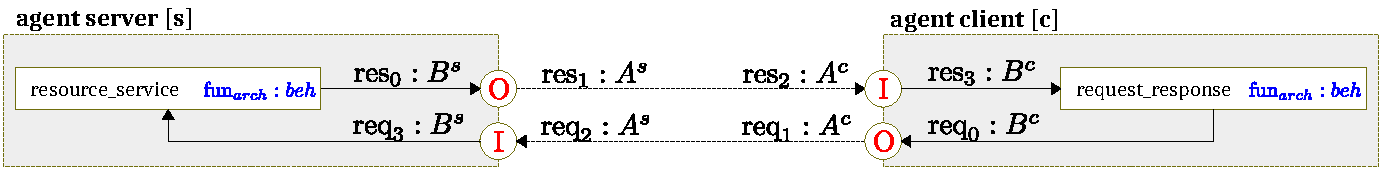
\includegraphics[width=\textwidth]{client-server.pdf}
	\caption{Client-Server paradigm in $\abf$-theory}
	\label{fig:client-server}
\end{figure}
Availability, again, is the denial of use of a resource. In the $\abf$-theory, 
in order to prevent a resource to be available, there
exists only (i.e. inclusively) the following mutually exclusive cases
that we illustrate using a client-server paradigm (depicted in Figure~\ref{fig:client-server}).
\begin{enumerate}
	\item\label{case:srv1} The resource on the server cannot be found, so that it is
		possible for the client to contact the server and the server
		sends a response back, but the output-port does not receive the
		necessary information. This may be due to a software error such
		that the functional architecture doesn't output a response, or
		a problem in the flow of information (i.e. the functional
		architecture doesn't receive the necessary information from
		other resources), or an hardware failure \&c. This is formalized
		as the relation between the beliefs produced by the functional
		architecture and the ones received by the output port, i.e.
		$\rcc(\behaviorRegion_s,\{\text{res}\})$ or 
		$\rcc(\beliefRegion_s,\{\text{res}\})$ 
	\item\label{case:srv2} The server hosting the resource is down, and then the server
		cannot output responses (i.e. insecure output port due to drop-related issue) or receive
		requests (insecure input port due to drop-related issue) or both.
	\item The client cannot properly compute request (simmetrically to Case~\ref{case:srv1})
	\item The client is down, symmetric to Case~\ref{case:srv2}
	\item The channel is down due to a drop related issue in one of the two channels 
\end{enumerate}

\begin{definition}{\bf Infosec-Availability --}\label{def:infosec-c}
\end{definition}

\begin{definition}{\bf Agent-Availability --}\label{def:agent-a}
\end{definition}

\begin{definition}{\bf System-Availability --}\label{def:system-a}
\end{definition}

\begin{definition}{\bf Infosec-Confidentiality --}\label{def:infosec-c}
	An Information $\varphi$ is considered to be confidential to a set of 
	agents $Ag_c$ if, per each agent $a\in Ag_c$, the content of the
	information (i.e. the data it carries) can only be understood (i.e. the relation
	between the information and its data can be known) by the
	agents in $Ag_c$.

	\begin{itemize}
		\item[$(\interpretation21)$] for all agents $a\in Ag$,
			$\world\models\information{a}{\varphi}$ and
			$\world\models\rcc(\varphi,Conf) \wedge
			\neg\dr{Conf}{\varphi}$ iff for any world $\world'$
			such that $\world \modalrelation\world'$,
			$\world'\models\believe{a}{\varphi}$, and
			$\world'\models\knows{a}{\exists f.~
			f(\information{a}{\varphi})=\varphi}$, where 
			$Conf$ is a Region and $f$ is an uninterpreted function.
	\end{itemize}
\end{definition}

\begin{example}{Dummy security protocol --}
	The last part (part III) of the protocol in our first example
	(Figure~\ref{fig:protocol-example}) represents the actual key exchange
	which, in general, needs to be confidential; otherwise the key would be
	known by any other agent who can, e.g., read on the communication
	channel.  Therefore, the last message, in Alice-and-Bob notation can be
	rephrased as: \begin{displaymath} Alice\Rightarrow Bob: enc(pk(Bob),
	symmetricKey) \end{displaymath} where $enc$ is the standard asymmetric
	encryption operator that encrypts the message $symmetricKey$ with the
	public key of Bob $pk(Bob)$ (see, e.g.,
	\autocite{Rocchetto2017interpolation} for a detailed formalization).
	The function $f$ in Definition~\ref{def:infosec-c}, represents any
	function used to enforce confidentiality on information.  In this
	example, $f$ is identified with $enc$ (i.e.
	$enc(pvt(Bob),symmetricKey)=symmetricKey$), the information is
	$\information{Alice}{[enc(pk(Bob),symmetricKey)]}$ and the data, i.e.
	$\varphi$ in Definition~\ref{def:infosec-c}, is $\varphi=symmetricKey$.
	In the perfect cryptography assumption, and assuming for simplicity
	that the logic of the whole protocol preserves confidentiality, the
	message is confidential. In fact, if $Ag={Alice, Bob}$ and $\eq{symmetricKey}{Conf}$:
	\begin{align*}
		\world^0\models\belief{Alice}{symmetricKey},\\
		\world^1\models\information{Alice}{symmetricKey}, \text{and}\\
		\world^2\models\belief{Bob}{symmetricKey} ~\text{if} \\
		enc(pvt(Bob), \information{Alice}{symmetricKey}=symmetricKey)=symmetricKey\\
		(i.e. f=enc ~\text{and}~ \information{Alice}{symmetricKey}=enc(pub(Bob),symmetricKey))\\
	\end{align*}
\end{example}

\begin{definition}{\bf Agent-Confidentiality --}\label{def:confidentiality}
An agent preserves the property of confidentiality iff 
\end{definition}

\begin{definition}{\bf System-Confidentiality --}\label{def:confidentiality}
	The property of confidentiality holds in a system when its information
	preserves confidentiality.
\end{definition}


\fix{mr}{
Confidentiality: the information is accessible only to authorised individuals.
A set of rules that limits access to information.  The information can be
accessed by X if and only if X is authorized to access it = X has the right
attributes (i.e. keys, password) to access it.

Integrity: the information is trustworthy and accurate (i.e. uncorrupted and
unaltered). Protects data from modification or deletion by unauthorized sources
and the ability to undo any damage done.  (for data at rest) If the information
X is written, A will always be read. If information X is modified to
information X', information X can always be recovered.  (for data in transit)
If the information X is sent, A will be received. If information X is modified
to information X', information X can always be recovered.

Availability: the information is accessible and usable when required. Guarantee
of reliable access to the information by authorized people If the information X
needs to be accessed, information X can be retrieved. If

Authenticity: assurance that the information is from the source it claims to be
from. Authenticity involves proof of identity. Authenticity is verified through
authentication.  If information X arrives from A to B, A sent information X and
B can verify it.  ??Authenticity implies integrity but Integrity doesn't imply
authenticity??  ??Authenticity doesn't imply confidentiality but
confidentiality does imply authenticity??

Non-repudiation: the ability to ensure that a party to a contract or a
communication cannot deny the authenticity of their signature on information
(or the sending of) that they originated.  If information X arrives from A, A
sent it and cannot deny it (partial overlap??).  If sender A sends information
X, it cannot say he didn't do it.  Non-repudiation implies authenticity and
integrity. Authenticity doesn't imply non-repudiation (replay attacks?).
Integrity doesn't imply non-repudiation (replay attacks?). 
}
\subsection{Abstraction Level of a Specification in $\abf$-theory}
As highlighted in \autocite{}, ``The level of abstraction is always a concern
when it come sto the definition of a system model.'' (as we already mentioned in Section~\ref{sec:problem}).

